\documentclass[12pt]{article}

\usepackage[]{amsmath}
\usepackage[]{amsthm}
\usepackage[]{amsfonts}
\usepackage[]{amssymb}
\usepackage{blindtext}
\usepackage[a4paper, total={6in, 8in}]{geometry}

\usepackage{listings}
\usepackage{color}

\definecolor{dkgreen}{rgb}{0,0.6,0}
\definecolor{gray}{rgb}{0.5,0.5,0.5}
\definecolor{mauve}{rgb}{0.58,0,0.82}
\usepackage{graphicx}
\graphicspath{ {/home/dimitri/Desktop/School stuffs/EECS3221/assignments/a2} }

\lstset{frame=tb,
  language=C,
  aboveskip=3mm,
  belowskip=3mm,
  showstringspaces=false,
  columns=flexible,
  basicstyle={\small\ttfamily},
  numbers=left,
  numberstyle=\small\color{black},
  keywordstyle=\color{blue},
  commentstyle=\color{dkgreen},
  stringstyle=\color{mauve},
  breaklines=true,
  breakatwhitespace=true,
  tabsize=4
}



\title{EECS3221 Assignment 2 report}
\author{Jerry Wu (217545898)}
\date{Due 07/31/2023}

\begin{document}

\maketitle

\section*{Abstract}
In this paper, I will be discussing varying topics relating to the \textbf{Sega Genesis} game console. Topics include, but are not limited to the type of operating system the console uses, OS architecture, kernel supports, etc.

\section{The operating system}

The Sega Genesis, originally known as the Sega Mega Drive, used a proprietary operating system known as SegaOS developed in 1988 by Sega when the console was first introduced to consumers in Japan.

\section{System architecture}
SegaOS follows a monolithic kernel architecture. All operating system services and functionalities are packed into a single large executable image that runs in kernel mode. This design choice was suitable for the Sega Genesis platform due to its relatively simple hardware and low memory constraints.

\subsection*{Pros and cons of monolithic architecture}
By having all the services within a single kernel, the system can achieve better performance as there are fewer context switches between different kernel components. However, the downside is that if there is a bug or failure in one part of the kernel, it can potentially crash the entire system. Nevertheless, for a gaming console like the Sega Genesis where the hardware is consistent and optimized for gaming, a monolithic kernel was a sound choice for the tech that was available at the time.


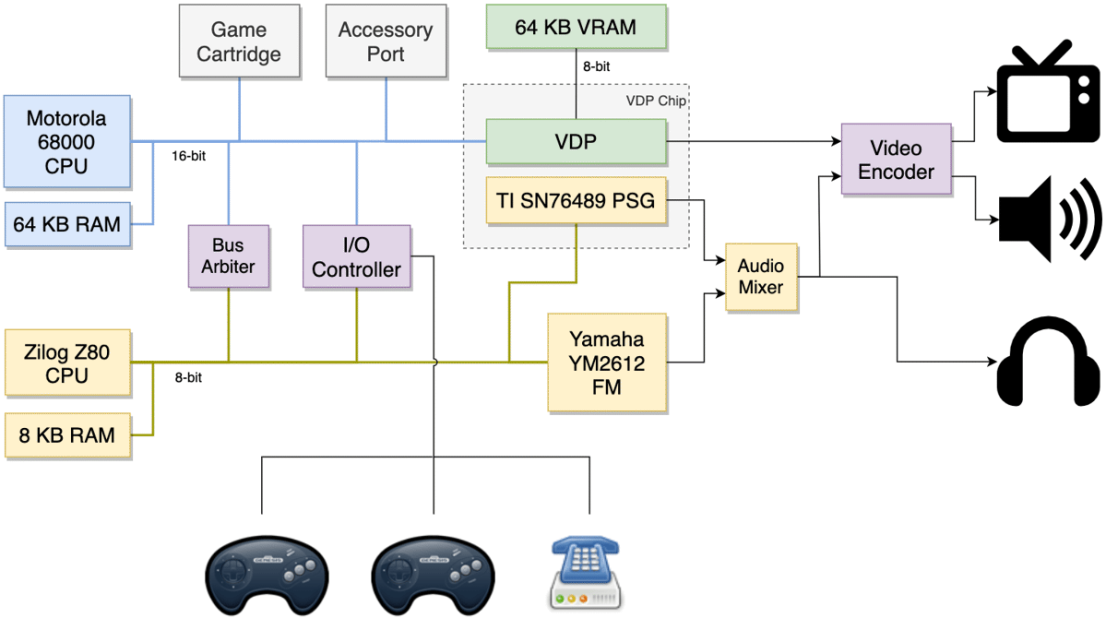
\includegraphics[width=0.8\textwidth]{diagram}
\\A system architecture diagram of the Sega Genesis (copetti.org)


\section{The boot sequence}
The following list of steps describes the boot sequence of the Sega Genesis:

\begin{itemize}
  \item[1.] When the console is powered on, the system initializes essential hardware components, including the CPU, RAM, and other system peripherals.
  \item[2.] The system then loads the initial boot code from a read-only memory (ROM) chip, commonly known as the BIOS (Basic Input/Output System). The BIOS is responsible for performing basic system checks, initializing some hardware, and preparing the system for the main operating system.
  \item[3.] Once the BIOS completes its tasks, it loads the main operating system, SegaOS, from the game cartridge or external storage media (e.g., floppy disk or CD-ROM).
  \item[4.] After SegaOS is up and running, it takes control of the system, manages memory, and provides services to games and applications.
\end{itemize}
\newpage
\section{Multithreading and concurrency?}
Because the system came out in 1998, the very concept of multitasking and multithreading was out of the question, as technology of that time was too primitive to handle such a task. Only single tasks are supported due to hardware limitations; once a game is run, the system will only be running that game and nothing else can run alongside it or be switched to from the game that is already running.

\section{CPU architecture}
The Sega Genesis uses a Motorolla 68000 series CPU, which is a 16 bit CPU. This CPU utilizes the RISC architecture. Interrupt handling on the Sega Genesis involves the CPU responding to hardware interrupts generated by both internal hardware and peripherals, such as controllers, timers, or other I/O operations. When an interrupt occurs, the CPU suspends the current task it is executing, saves its context, and jumps to the interrupt service routine specified for that particular interrupt. After the routine is completed, the CPU resumes the previous task from where it left off.

\section{Creation and deployment of new software}
Creating and deploying a new program for the Sega Genesis typically involves using a specific software development kit (SDK) provided by Sega or third-party developers. This SDK includes tools, libraries, and documentation to aid developers in creating games and applications.

\subsection*{Programming Language} 
Developers who wish to create new software for the Sega Genesis can do so with the RISC based assembly language or use higher-level languages such as C or C++. Assembly was often preferred for performance-critical sections, while C and C++ provided a more developer friendly experience, as it enabled easy readability.
\\
\newpage
Here is an assembly example of creating a colour palette and loading it into the console's memory provided by Hugues Johnson from his guide on Sega Genesis programming:

\subsection*{Creating the palette}
\begin{lstlisting}
PaletteWinter:
dc.w	$0F0F	; rgb(240,000,240) => 1111 0000 1111 => 0F0F
dc.w	$0115	; rgb(080,048,032) => 0010 0011 0101 => 0115
dc.w	$0356	; rgb(096,080,048) => 0011 0101 0110 => 0356
dc.w	$0139	; rgb(144,096,016) => 0001 0011 1001 => 0139
dc.w	$0031	; rgb(016,048,000) => 0000 0011 0001 => 0031
dc.w	$0033	; rgb(048,048,000) => 0000 0011 0011 => 0033
dc.w	$0FEE	; rgb(224,224,240) => 1111 1110 1110 => 0FEE
dc.w	$0FED	; rgb(208,224,240) => 1111 1110 1101 => 0FED
dc.w	$0FEC	; rgb(192,224,240) => 1111 1110 1100 => 0FEC
dc.w	$0ECD	; rgb(208,192,224) => 1110 1100 1101 => 0ECD
dc.w	$0FFF	; rgb(240,240,240) => 1111 1111 1111 => 0FFF
dc.w	$0EED	; rgb(208,224,224) => 1110 1110 1101 => 0EED
dc.w	$0ABB	; rgb(176,176,160) => 1010 1011 1011 => 0ABB
dc.w	$0358	; rgb(128,080,048) => 0011 0101 1000 => 0358
dc.w	$0345	; rgb(080,064,048) => 0011 0100 0101 => 0345
dc.w	$0DCC	; rgb(192,192,208) => 1101 1100 1100 => 0DCC
\end{lstlisting}
\newpage
\subsection*{Loading the palette into memory}

\begin{lstlisting}
;---------------------------------------------------------------------
; LoadPalette
; a0 = address of first palette to load
; d0 = number of palettes to load (1-4)
;---------------------------------------------------------------------
LoadPalette:
  move.l	#$C0000000,($00C00004) ; set up VDP write to CRAM
  mulu	#$10,d0	; multiply number of palettes by 16
  sub.w	#$01,d0	; subtrack 1 since the loop counts to 0
LoadPaletteLoop:
  move.w	(a0)+,($00C00000)	; write the palette data
  dbf	d0,LoadPaletteLoop		; decrement value of d0 and loop if not 0
  rts
\end{lstlisting}

\subsection*{Compilers, Linkers, and Loaders} 
The SDK includes a compiler to translate high level source code into assembly code that the Sega Genesis can execute. It also includes a linker that is used to combine compiled code with other necessary assets for game development such as graphics and sound effects into a single executable file that can later be put onto a cartridge. The loader within the SDK is responsible for loading the program from the cartridge or storage medium into the system's memory.


\section{Porting from Sega Genesis to Windows?}
Porting a program from the Sega Genesis to a PC running Windows 10 involves significant challenges due to the differences in hardware architecture, operating systems, and programming paradigms.

\subsection*{Steps for Porting}

\begin{itemize}

\item[1.] \textbf{Understanding the Original Code}: Analyze the existing game's source code and assets to understand its architecture, dependencies, and any hardware-specific optimizations.

\item[2.] \textbf{Rewriting or Adapting Code}: Since the Sega Genesis used a 16 bit CPU with specific hardware features, a considerable portion of the code will need to be rewritten or heavily adapted to work on modern 32/64-bit x86 CPUs.

\item[3.] \textbf{Graphics and Audio}: The graphics and audio subsystems of the Sega Genesis are vastly different from modern PCs. Graphics libraries, APIs, and audio engines need to be re-implemented or replaced with PC-compatible ones.

\item[4.] \textbf{Input Handling}: The game's input handling will need to be adapted to work with PC peripherals like keyboards, mice, or game controllers.
Testing and Debugging: Rigorous testing and debugging are essential to identify and fix issues arising from platform-specific differences.

\item[5.] \textbf{Porting vs. Emulating}:
Porting involves rewriting or adapting the program's source code to run natively on the target platform, while emulation involves running the original program (ROM) through an emulator software that mimics the Sega Genesis hardware on the PC. Emulation can be quicker to set up but may not provide the same performance or accuracy as a native port.

\end{itemize}

\section{Using a different OS other than SegaOS?}

Deploying a different operating system, such as Linux or Windows, onto the Sega Genesis would be an extensive and challenging task due to the hardware and firmware limitations of the console.

\subsection*{Steps for Deploying a Different OS}
\begin{itemize}
\item[1.]\textbf{Hardware Compatibility}: We must first ensure that the chosen operating system is supported by or can be adapted to work with the Sega Genesis hardware components, including the 16 bit 68000 CPU, memory, graphics, and audio.

\item[2.]\textbf{Bootloader or Firmware Modification}: To run a different operating system, the console's existing bootloader or firmware may need to be modified or replaced with one compatible with the new OS.

\item[3.]\textbf{Device Drivers and Kernel Customization}: We need to develop or adapt device drivers for the Sega Genesis hardware to enable proper interaction with the new operating system to ensure no hardware failures occur because of the new OS.

\item[4.]\textbf{File System and Storage}: We also need to implement or modify the file system to work with the storage medium (e.g., cartridge, floppy disk) used by the Sega Genesis.

\item[5.]\textbf{Memory Constraints}: The limited hardware capabilities of the Sega Genesis could hinder the performance of a modern operating system, potentially making it impractical or significantly reducing its functionality.
Porting a modern operating system may require external memory expansions or other hardware modifications, which may not be easily achievable or practical for the platform.
\end{itemize}

Needless to say, the concept of loading a modern OS like Windows 10 or Linux Mint onto a Sega Genesis is absurd at best, as the 1988 hardware limitations of the system make it more work than it is worth.

\newpage
\begin{thebibliography}{9}

\bibitem{texbook}
Sega Enterprises, Ltd. "Sega Genesis Instruction Manual." 1989.

\bibitem{lamport94}
Sega Enterprises, Ltd. "Genesis II/Mega Drive II Service Manual." 1993.

\bibitem{website}
H. Johnson, “Speedrun Tower” HuguesJohnson.com, 2000-2023

\bibitem{website}
R. Copetti, “Mega Drive/Genesis Architecture: A practical analysis” The Copetti site, https://www.copetti.org/writings/consoles/mega-drive-genesis/ (accessed Jul. 31, 2023). 

\end{thebibliography}



\end{document}